%----------------------------------------
% Preamble to set up the document
%----------------------------------------
\documentclass{article}

% set up packages (you shouldn't need to touch this)
\usepackage{graphicx}  % required to insert images
\usepackage{hyperref}  % for hyperlinks
\usepackage[svgnames]{xcolor}  % to change hyperlink colors
\colorlet{linkcolour}{DarkBlue}
\hypersetup{colorlinks=true, linkcolor=linkcolour, citecolor=linkcolour, urlcolor=linkcolour,}

% Margins
\topmargin=-0.45in
\evensidemargin=0in
\oddsidemargin=0in
\textwidth=6.5in
\textheight=9.0in
\headsep=0.25in

% use a sans serif font
\renewcommand{\familydefault}{\sfdefault}

%----------------------------------------
% Step 1: Edit the lecture title
%----------------------------------------
\title{
Lecture 3: Computational Complexity \\  % Lecture title
Modeling Social Data, Spring 2018 \\   % Course title
Columbia University                    % School
}

%----------------------------------------
% Step 2: Edit your name and the date
%----------------------------------------
\author{Nancy Thomas}                     % Scribe's name
\date{February 8, 2018}                % Lecture date

\begin{document}

\maketitle


%----------------------------------------
% Step 3:
% Rename uni.tex to match your uni,
% edit the filename accordingly below,
% and put your notes in this file
%----------------------------------------
%----------------------------------------
% Write your notes here
%----------------------------------------

\section{Part 1: Guest Lecture}
The first part of class was a guest lecture by Sidharth Sen, who works with Jake at Microsoft Research here in NYC. Sid's research focuses on algorithms and systems and networking and Jake noted that one of his more notable research topics involved weak AVL trees. Sid's background has a large data structures influence, and his lecture focused on exploring the question of how to store and manipulate data and how long things take.

\vspace{3mm}
Sid's aim for the lecture was to explore the following four topics:
\begin{enumerate}
    \item Computational tractability
    \item Asymptotic order of growth
    \item Common running times (data structures, algorithms)
    \item Applications
\end{enumerate}

\subsection{Computational Tractability}

We started by roughly defining computational tractability as how to tell how long things take. Another term associated with this idea is running time, T(n), which we take to be a function of the input size n. Sid highlighted some examples of common running times. Here, it is important to note that in general, constants do not matter. In other words, we will take $2n$ to be the same as $n$ since we are most interested in asymptotic behavior. The examples are as follows:

\begin{itemize}
    \item $2^n$
    \begin{itemize}
        \item exponential
        \item not good
        \item often happens with a brute force search or in a situation when we try all combinations of something
    \end{itemize}
    \item $cd^n$ where $c, d > 0$ are constants
    \begin{itemize}
        \item polynomial
        \item not good when we are working with big data
        \item theoretical computer scientists often consider this to be ok
        \item here we do have to pay attention to the constants at least a little because it is not always obvious which algorithm is worse (ie. $20n^{100}$ versus $n^{1+0.002\logn}$)
    \end{itemize}
    \item n
    \begin{itemize}
        \item linear
        \item good
    \end{itemize}
    \item $\log(n)$
    \begin{itemize}
        \item logarithmic
        \item sublinear which means we don't need to look at all of the data in a set, sometimes this means that data preprocessing is involved
        \item good
    \end{itemize}
    \item c where $c>0$ is a constant
    \begin{itemize}
        \item constant
        \item no n dependence
        \item good
    \end{itemize}
\end{itemize}

\subsection{Asymptotic Order of Growth}
Next, we moved on to looking at asymptotic order of growth, which is often expressed with big O notation. Here, Sid defined the analysis of run time in terms of:
\begin{itemize}
    \item worst case
    \begin{itemize}
        \item analyze how fast an algorithm runs when we have the worst possible input
    \end{itemize}
    \item average case
    \begin{itemize}
        \item analyze how fast an algorithm run on average when we  draw input from a random distribution 
    \end{itemize}
    \item amortized
    \begin{itemize}
        \item analyze how fast an algorithm runs when there is one big operation that happens infrequently
        \item considers an algorithm's run time based on the run time and frequency of individual operations
        \item Sid emphasized that it is often more optimal in many algorithms to perform an expensive operation infrequently than a slightly less expensive operation frequently
        \item an example of this is when reallocating an array it is better to double the size of the array each time the array needs to be reallocated so that we can insert elements into the array frequently without needing to reallocate space (an expensive operation) and we only need to reallocate infrequently
    \end{itemize}
\end{itemize}
\vspace{3mm}
Before diving into a more in depth analysis of big - O notation, Sid noted that in terms of speed, run times are ranked as follows: $n < n\logn < n^2 < n^3 < {1.5}^n < 2^n <n!$. This is important to keep in mind when considering upper and lower bounds.

\begin{figure}[h!]
  \begin{center}
    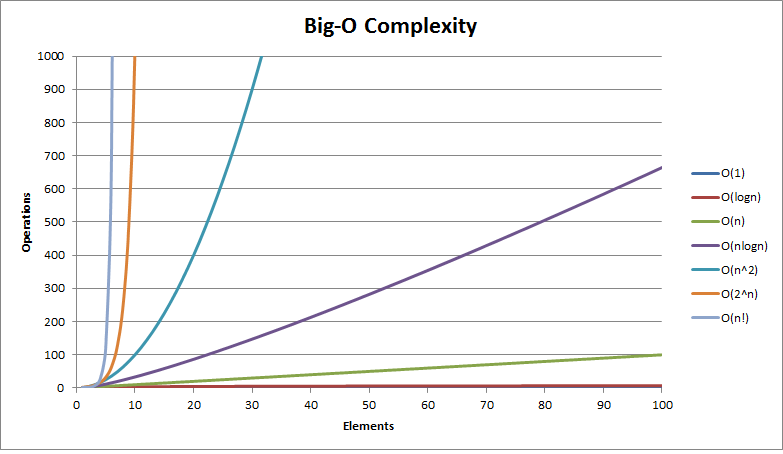
\includegraphics[width=0.5\textwidth]{figures/big-o-complexity.png}.
    \caption{
      Run time visual comparison (from http://www.kestrelblackmore.com/blog/big-o-notation-complexity)}
    \label{fig:example_figure}
  \end{center}
\end{figure}


\vspace{3mm}

For each of these types of run time analysis (worst case, average case, and amortized), we can consider three ways of expressing the run time:
\begin{enumerate}
    \item Upper bound \\
    
    The upper bound is defined as $T(n) = \mathcal{O}(f(n))$ if $\exists$  $c > 0, n_0>0$ st. $T(N) \leq cf(n)$  $\forall$  $n>n_0$. \\

\begin{figure}[h!]
  \begin{center}
    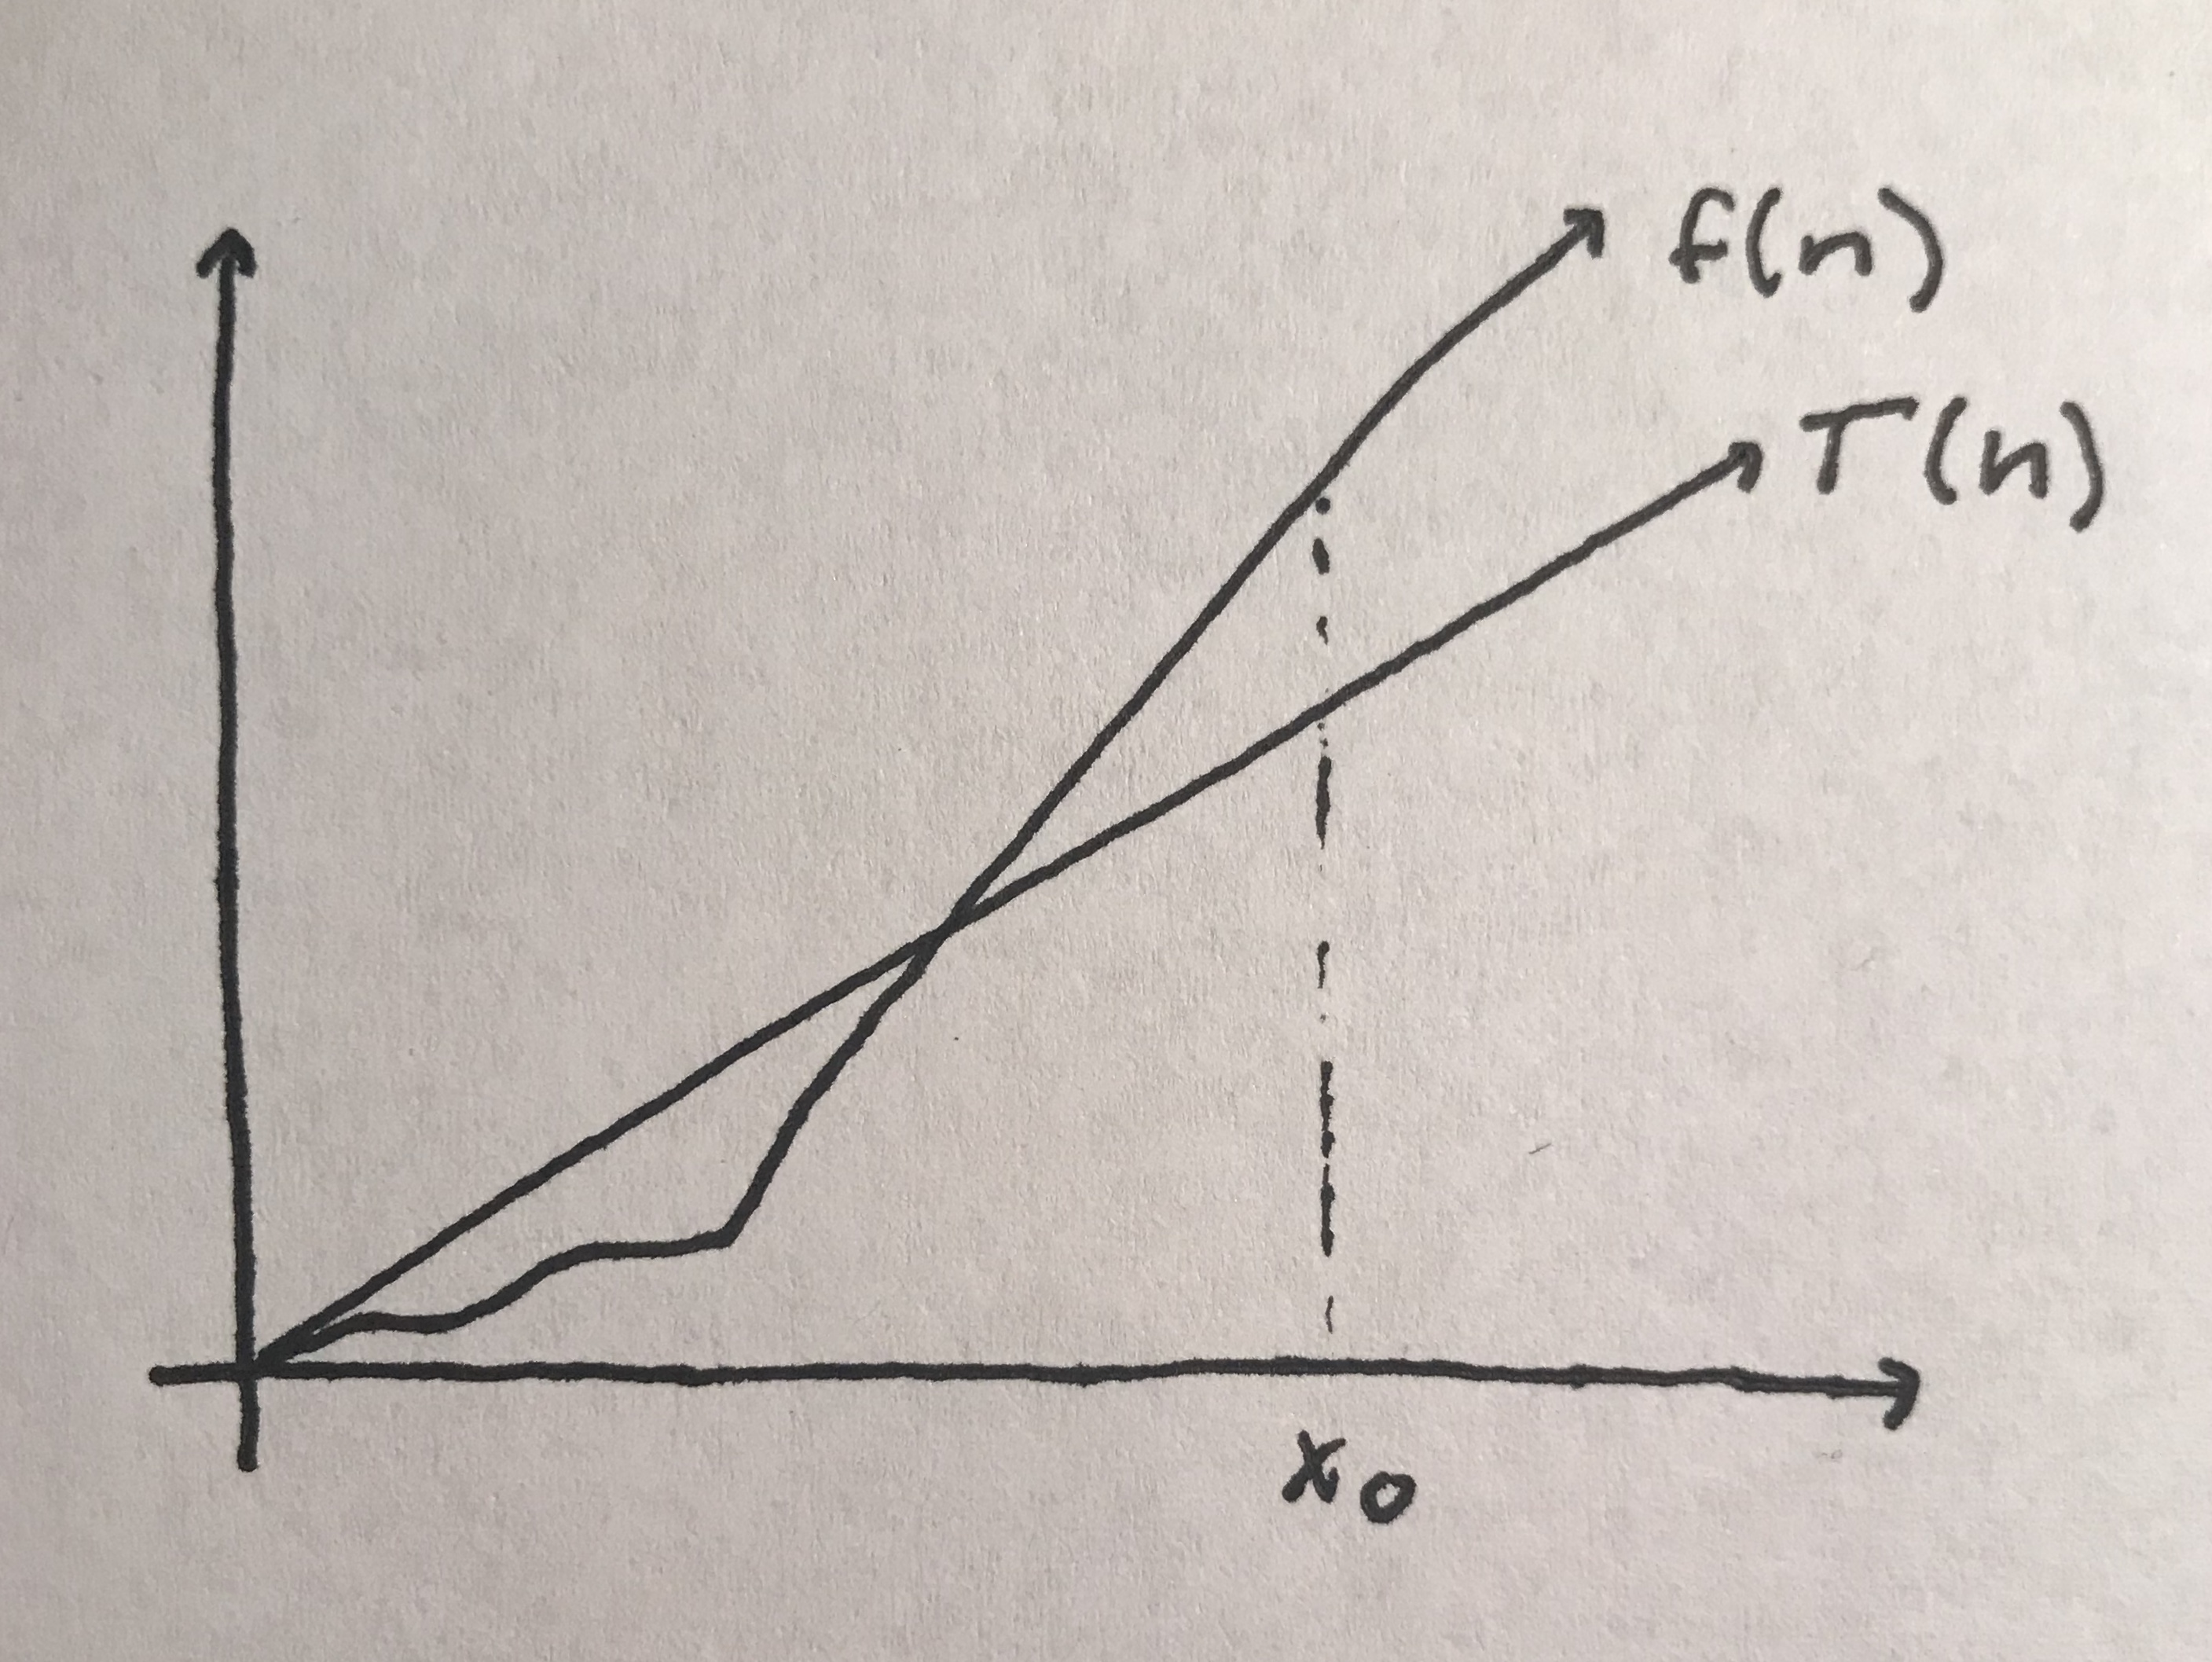
\includegraphics[width=0.4\textwidth]{figures/IMG_8828.jpg}.
    \caption{
      Upper bound visual representation}
    \label{fig:example_figure}
  \end{center}
\end{figure}
    
    ex. For example, if we have $T(n)=32n^2+17n+1$ we can say $T(n) = \mathcal{O}(n^2)$. This is evident because we could take $c=50$ and $n_0 = 1$. It is clear that in this case $T(n) \leq 50n^2$ when $n>1$ so $\mathcal{O}(n^2)$ is a good upper bound. It is also important to note here that we could in theory also say that $n!$ is an upper bound for this problem, but this result is not as interesting and does not give us as much information about the algorithm. Thus, it is best to select the lowest upper bound.
    
    \item Lower bound \\
    
    The lower bound is defined as $T(n) = \Omega(f(n))$ if $\exists$  $c > 0, n_0>0$ st. $T(N) \geq cf(n)$  $\forall$  $n>n_0$. \\
    
    \begin{figure}[h!]
  \begin{center}
    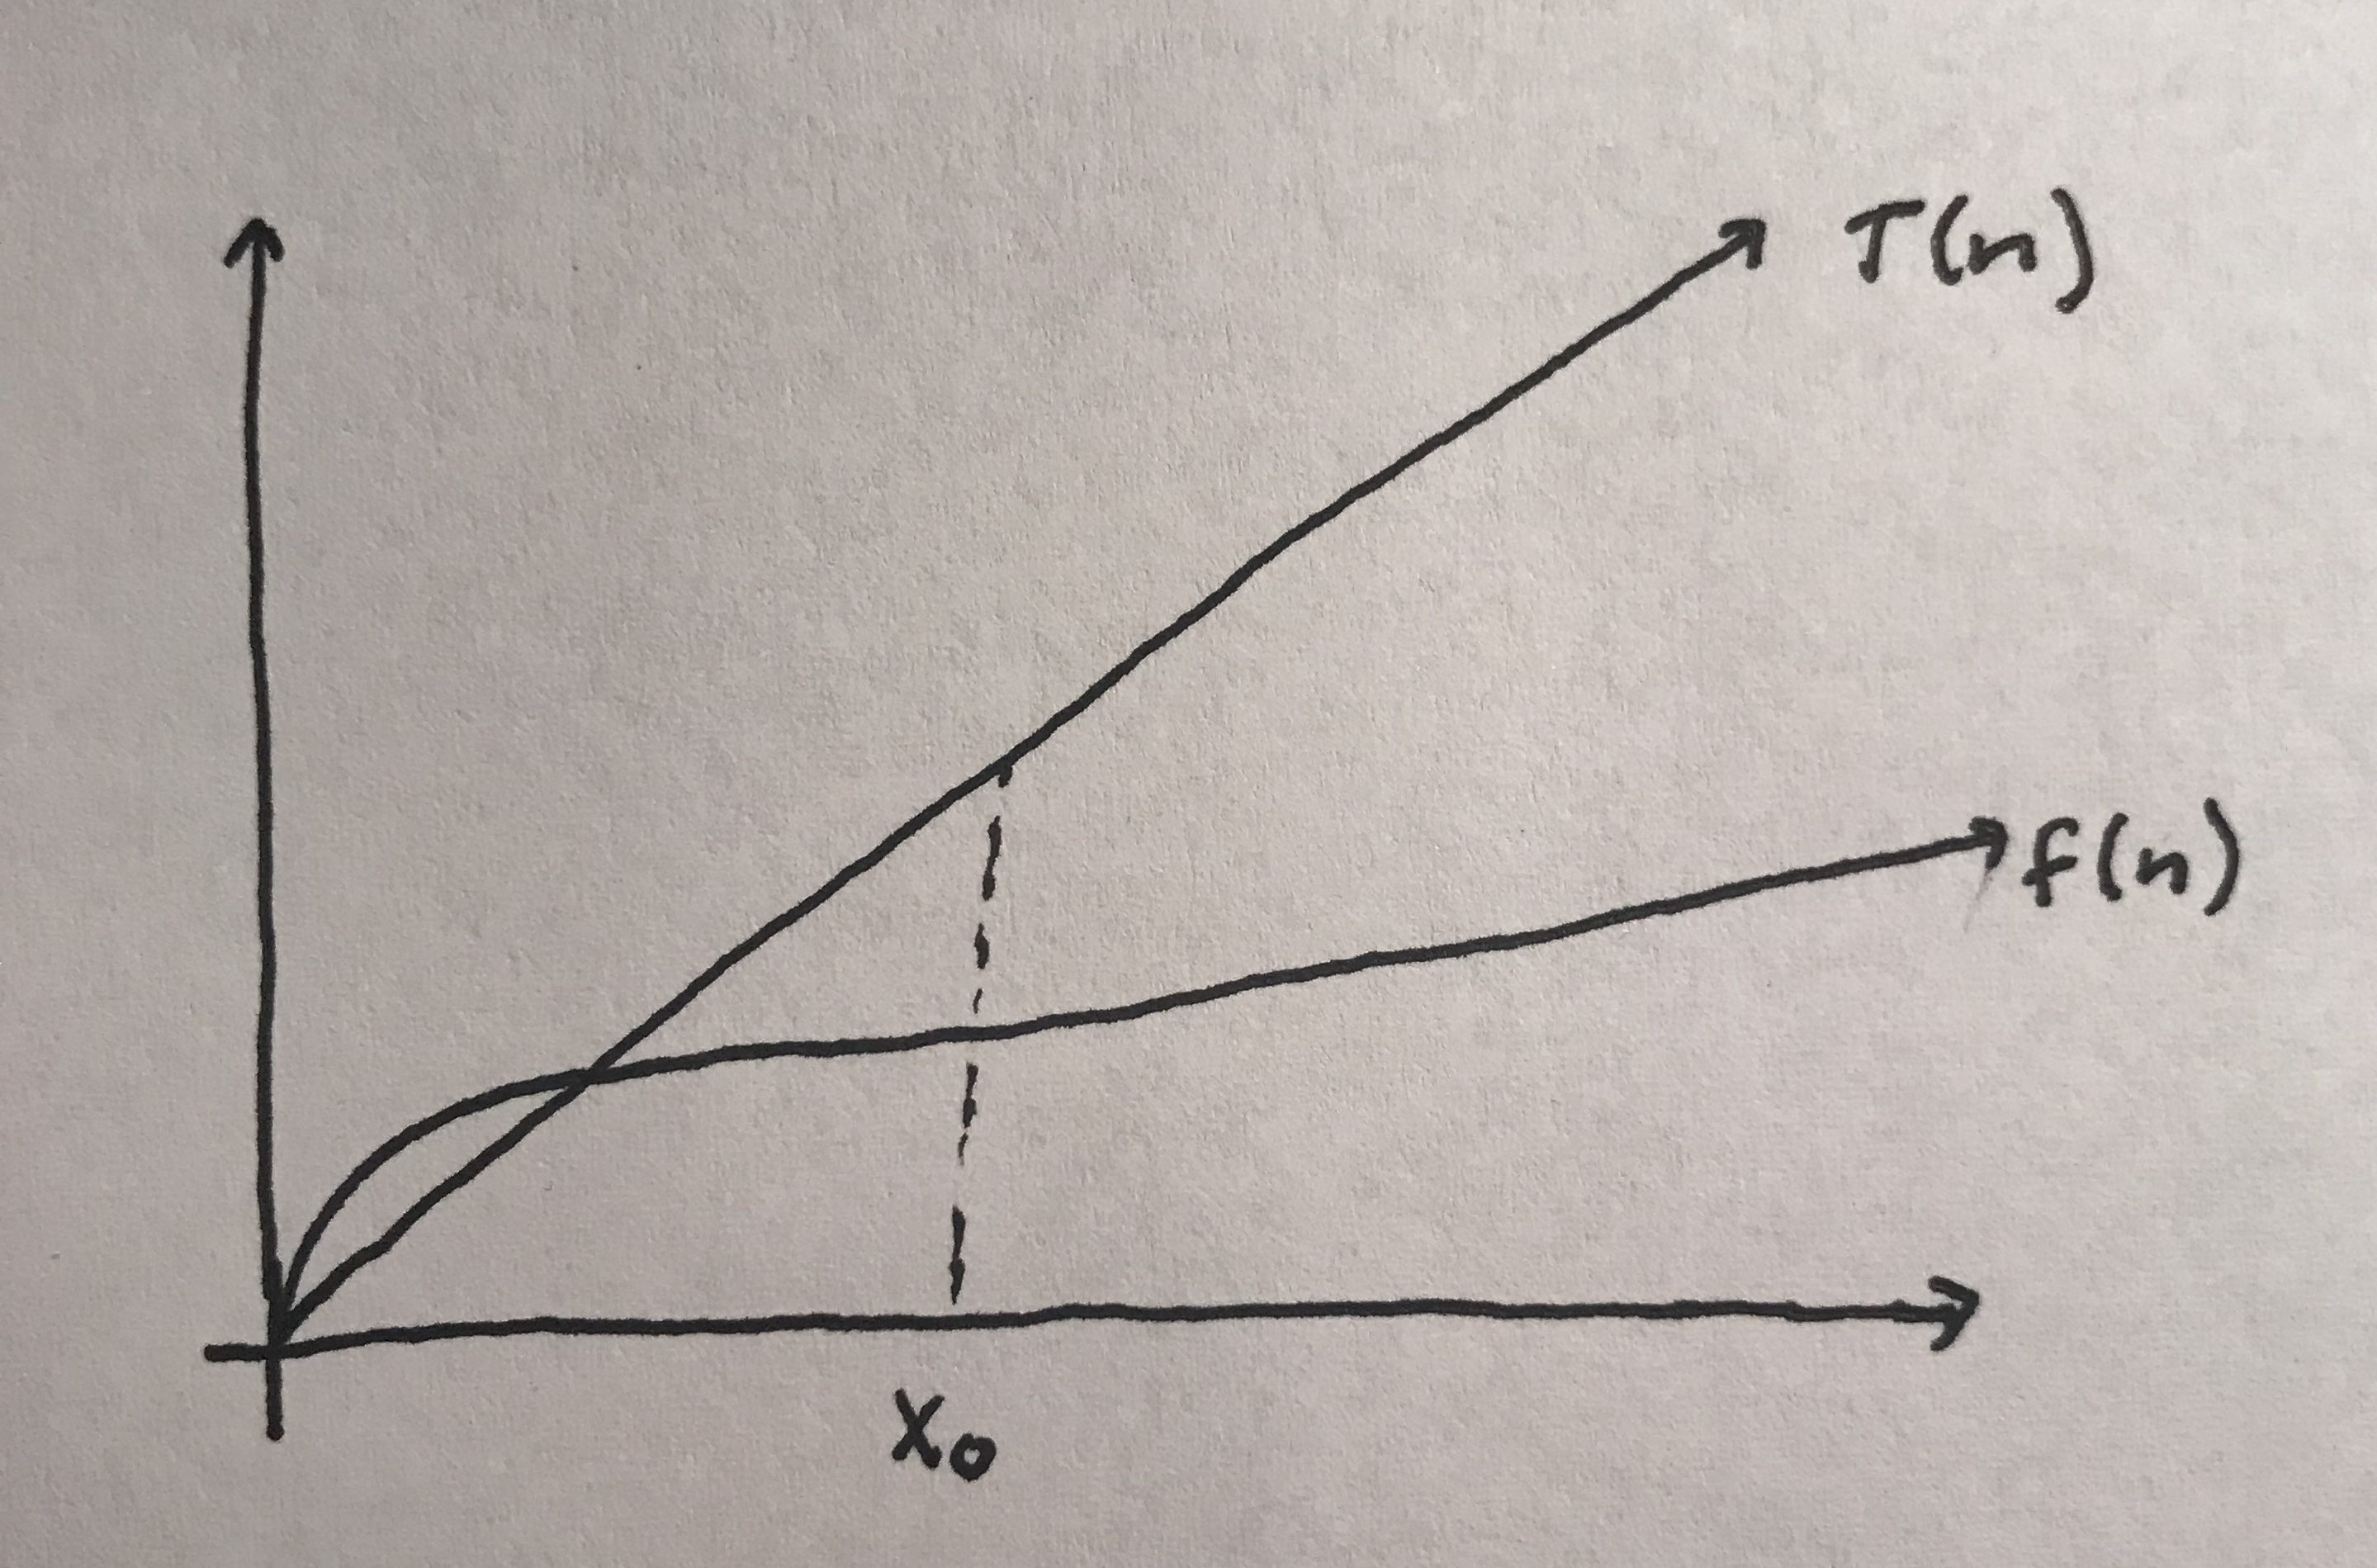
\includegraphics[width=0.4\textwidth]{figures/IMG_8827.jpg}.
    \caption{
      Lower bound visual representation}
    \label{fig:example_figure}
  \end{center}
\end{figure}
    
    ex. Let us again take the example $T(n)=32n^2+17n+1$. We can again take $T(n) = \Omega(n^2)$. For this case, we could take $c=1$ and $n_0 = 1$. It is clear that $T(n) \geq n^2$ when $n>1$ so $\Omega(n^2)$ is a good lower bound. Similarly to with the upper bound, it is best to choose the greatest lower bound. For example, saying $\Omega(1)$ does not tell us as much about the algorithm as $\Omega(n^2)$.
    
    \item Tight bound
    
    The tight bound is expressed as $T(n) = \Theta(f(n))$ if $T(n) = \mathcal{O}(f(n))$ and $T(n) = \Omega(f(n))$ and $\Omega(n) = \mathcal{O}(n)$. The visual representation for this bound is given by Figure 4.
    
     \begin{figure}[!]
        \begin{center}
            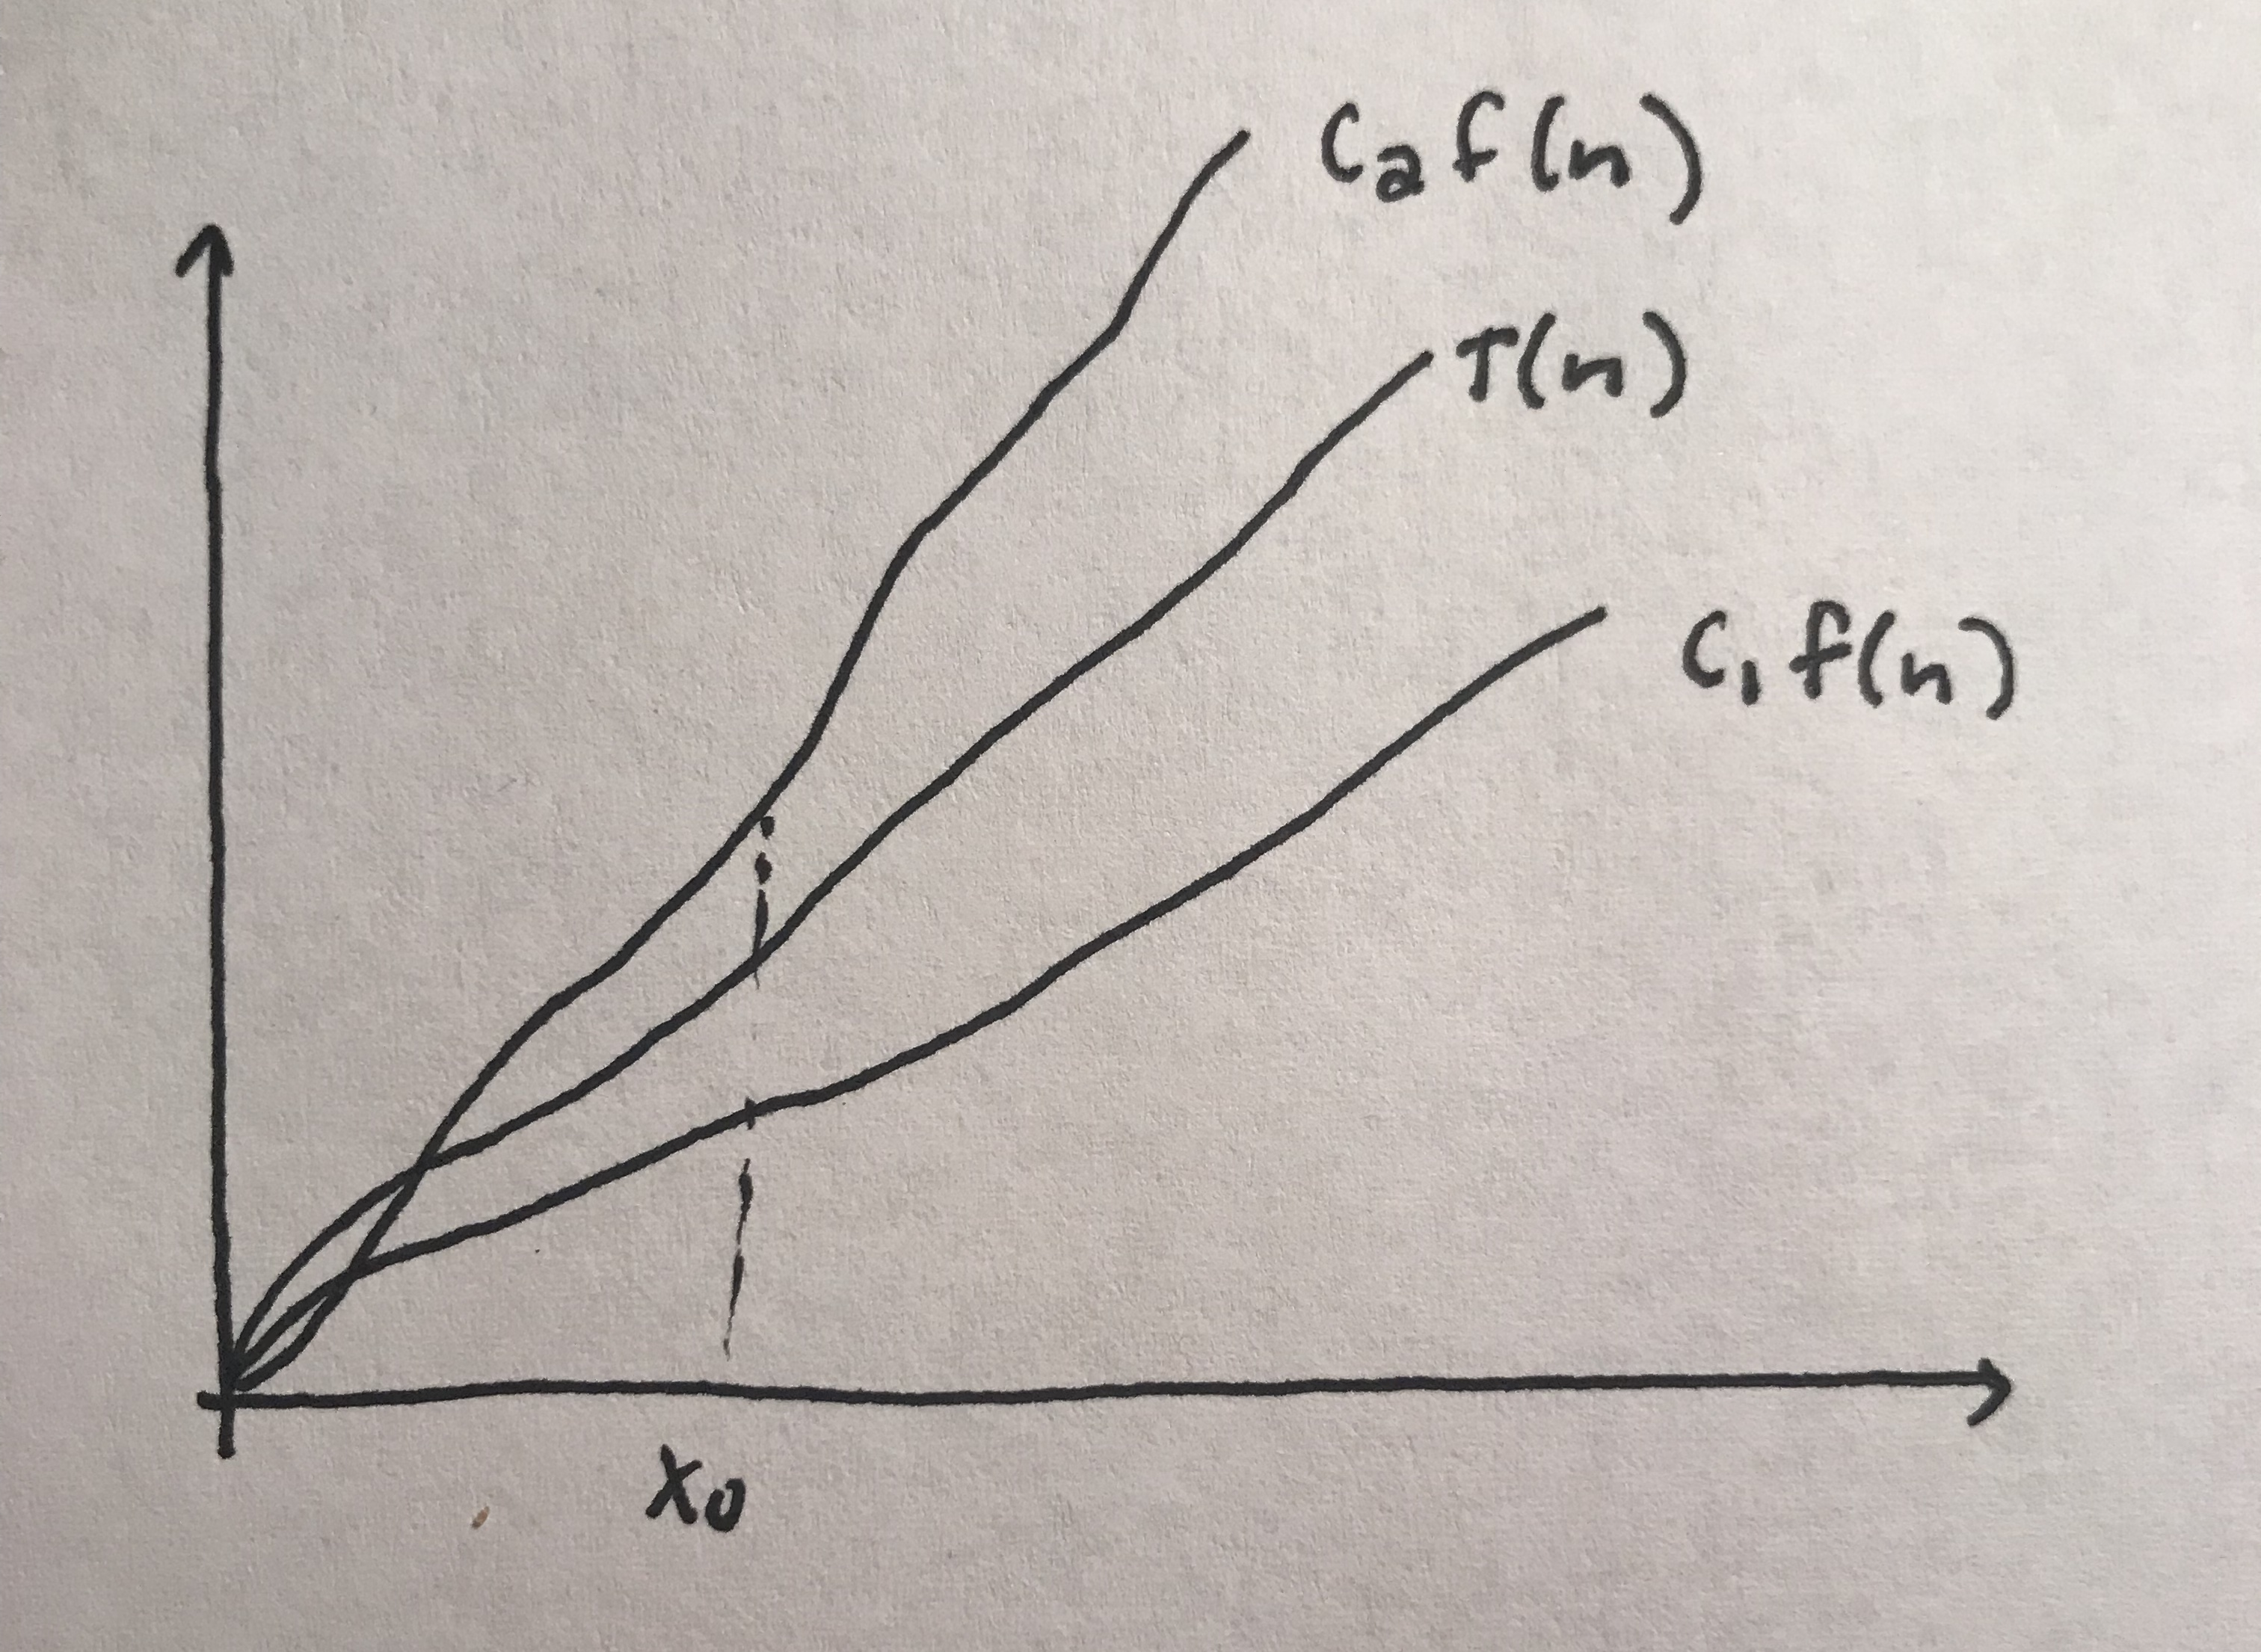
\includegraphics[width=0.4\textwidth]{figures/IMG_8826.jpg}.
            \caption{
            Tight bound visual representation}
        \label{fig:example_figure}
    \end{center}
    \end{figure}
    
    This can further be written as:
    $c_1f(n) \leq T(n) \leq c_2f(n)$ $\forall$ $n \geq n_0$ and $c_1, c_2 > 0$
    
    ex. In the example $T(n)=32n^2+17n+1$, we can say $T(n) = \Theta(n^2)$. The upper and lower bounds are also $n^2$. We can take for example $c_1 = 1$ and $c_2 = 50$ and $n_0 = 1$ and can see that $n^2 \leq T(n) \leq 50n^2$ when $n>1$.
\end{enumerate}

Next, Sid highlighted some "Rules of Thumb" when considering these upper, lower, and tight bounds:

\begin{enumerate}
    \item $T(n)=a_0 + a_1n + a_2 n^2 + \ldots + a_dn^d = \mathcal{O}(n^d) = \Omega(n^d) = \Theta(n^d)$
    \item $\mathcal{O}(\log_a n) = \mathcal{O}(\log_b n)$ for $a, b >0$ (base does not matter, it is another constant)
    \item $n^d = \mathcal{O}(r^n)$ $\forall$ $r>1, d>0$
\end{enumerate}

\subsection{Common Running Times}
Next, Sid walked through some common running times and gave examples of algorithms and data structures where these running times are commonly seen. It is important to note that here, we will assume that arithmetic, indexing, and "basic operations" take $\mathcal{O}(1)$ time. 

It is also essential to note something that has been absent from our discussion up to this point, but which is essential to keep in mind. That is thinking about the amount of space we take up when implementing certain data structures or algorithms. There is often a trade off between space and time, and space is important to consider because even if an algorithm operates in sublinear time, it might require storage of massive amounts of data, which could be inefficient or even impossible. Here, we will proceed with some common running times but keep the space complexity in the back of our minds as well.

\begin{enumerate}
    
    \item $\mathcal{O}(\log(n))$ \\
    Logarithmic run time is often seen when working with binary search trees, which is a commonly used data structure that has an inherent sorting structure which makes it so we do not have to visit every node. For example, inserting or searching in a BST has logarithmic run time. \\
    
    \begin{figure}[h!]
  \begin{center}
    \includegraphics[width=0.4\textwidth]{figures/BSTSearch.png}.
    \caption{
      Binary Search Tree Visual (from https://www.geeksforgeeks.org/binary-search-tree-data-structure/)}
    \label{fig:example_figure}
  \end{center}
\end{figure}
    
    Another data structure whose associated algorithms often have this run time is a skip list. Sid noted that we can think of the skip list as a sort of multi-leveled linked list. If the bottom level has n nodes, the next level up will have $\frac{n}{2}$ nodes and the next level after that will have $\frac{n}{4}$ nodes. The pattern continues so that each subsequent layer has half as many nodes as the previous layer. This data structure makes searching more efficient because it is possible to start at the level that is farthest out, which is analogous to starting at the first/root node in the BST. Thus, the run time for searching, similar to for a BST is $\mathcal{O}(\log(n))$. \\
    
    \begin{figure}[h!]
  \begin{center}
    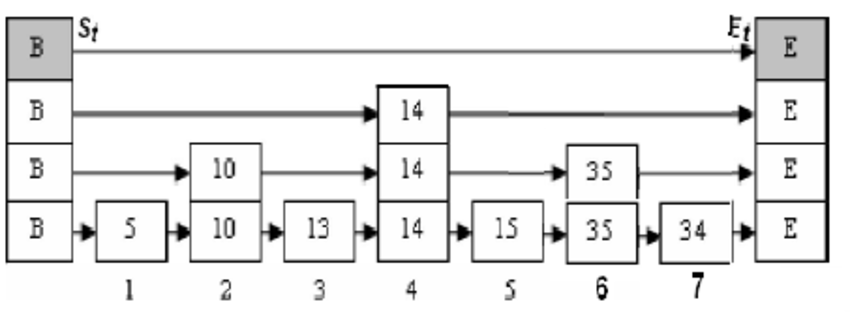
\includegraphics[width=0.5\textwidth]{figures/A-skip-list-is-a-set-of-linked-lists-Numbers-within-17-are-the-indexes-of-the.png}.
    \caption{
      Skip List Visual (from https://www.researchgate.net/figure/A-skip-list-is-a-set-of-linked-lists-Numbers-within-17-are-the-indexes-of-the_fig2_221560836)}
    \label{fig:example_figure}
  \end{center}
\end{figure}

    \item $\mathcal{O}(n)$ \\
    Linear run time is often seen when we need to touch each node or element only once. This might be the run time if we are searching for one element in a list of length n.
    
    \item $\mathcal{O}(n\log(n))$ \\
    
    A commonly seen algorithm with this run time is merge sort. It is also often seen in an algorithm where we have to touch every node in a layer, but the layers are organized in a manner like that in the skip-list where each subsequent layer has half the nodes of the preceding layer. For this algorithm, each layer takes $\mathcal{O}(n)$ time and there are $\log(n)$ layers (how many times n divides in half). This leads to an overall time complexity of $\mathcal{O}(n\log(n))$.
    
    \item $\mathcal{O}(n^2)$ \\
    
    Some commonly seen algorithms with this run time are bubble sort, quick sort, or any other algorithm where all pairs comparisons are made. More generally, this run time often results when the run time is $\mathcal{O}(n)$ per operation and we have to perform each operation $n$ times. It should be noted that the worst case run time for the quick sort algorithm is really bad if we are unlucky and start with the largest or smallest element as the pivot. \\
    
\end{enumerate}
    
We also briefly discussed a join algorithm, which we are likely to use in this course. This is used when we have two tables, each with an id and two different columns. Let us say table 1 has an id and then columns A and B while table 2 has the same id and columns C and D. The join algorithm produces a table with the id and columns A, B, C, and D. We discussed that the least efficient way to do this would take $\mathcal{O}(n^2)$ time if we searched each id in table 2. This could be improved to $\mathcal{O}(n\log(n))$ if we implement a sort of BST structure on the ids of column 2. The best method we uncovered, however, would take $\mathcal{O}(n)$ time and involves a hash table. We did not go into depth on what a hash table is but it was mentioned that lookups in a hash table take $\mathcal{O}(1)$ time. It is important when constructing a hash table that each bin does not get too large, otherwise the benefit of quick lookups is diminished.

\subsection{Applications}

Next, Sid discussed how some of the topics he discussed apply to things he is actually working on in his research. He is attempting to design a "Universal Data Structure."\\

\vspace{3mm}
Problem: The problem is that each data structure has its strengths and weaknesses. In other words, a data structure that performs well for inserts might perform very poorly for lookups and vice versa. This is an issue because when working on a problem, the workflow involves numerous different tasks, as depicted in the Figure 7, and it is difficult to choose a data structure that will perform optimally for most of the tasks. 

\\
\vspace{3mm}
Abstract solution: Sid's goal is to design a Universal Data Structure that can shape shift to have optimal performance at different phases of the workflow. This problem has not been solved yet, and it is something that Sid often asks his potential employees about in interviews.
\vspace{3mm}

 \begin{figure}[h!]
  \begin{center}
    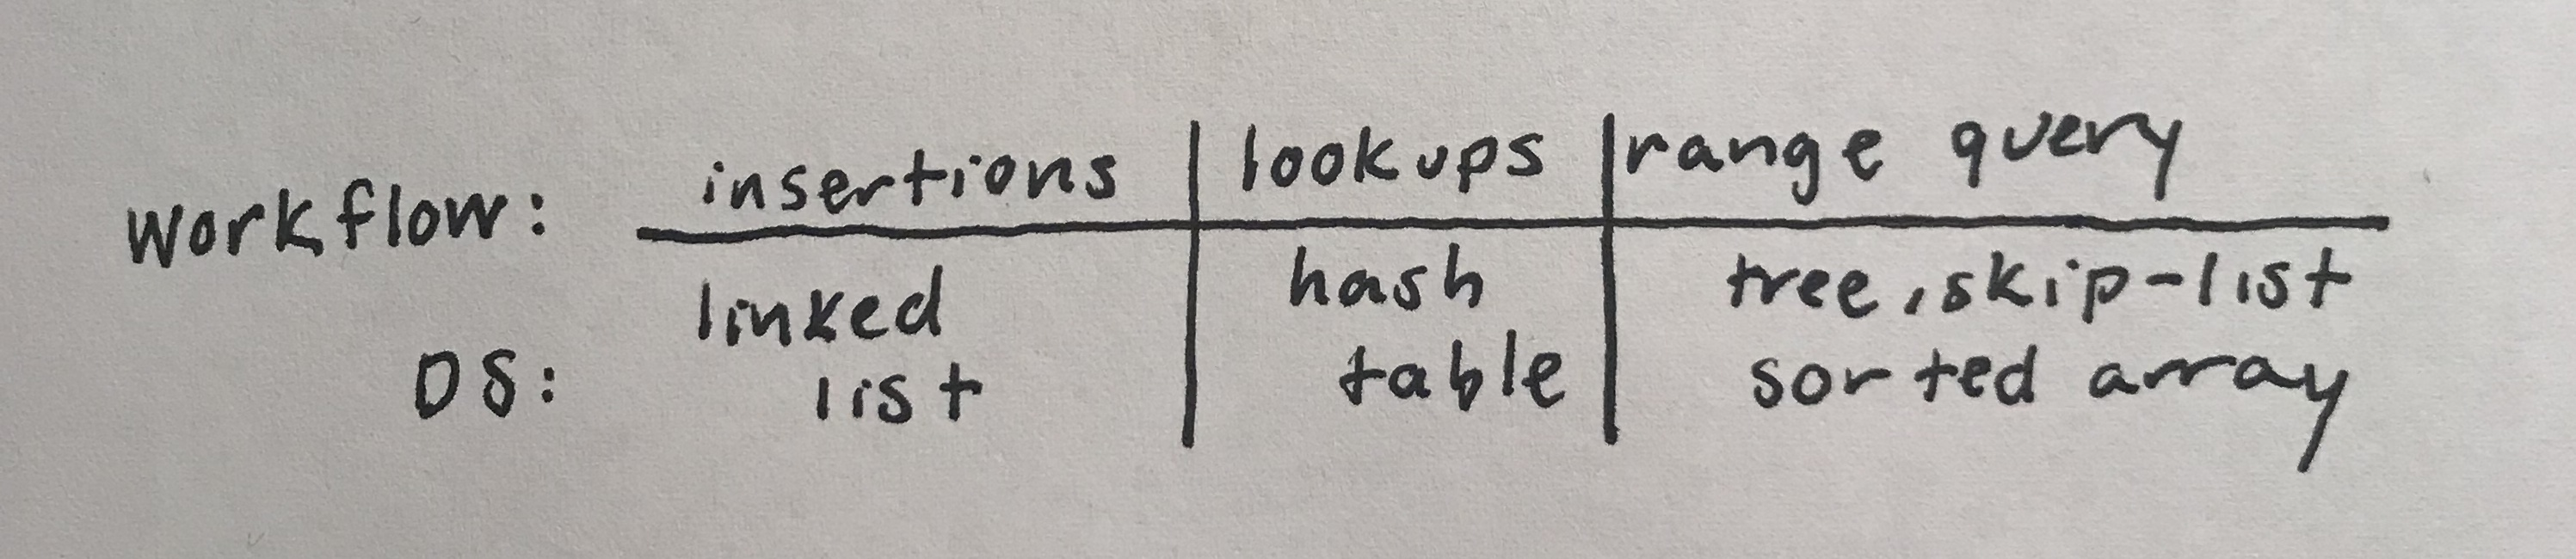
\includegraphics[width=0.5\textwidth]{figures/IMG_8829.jpg}.
    \caption{
      Workflow Diagram With Tasks and Associated Data Structures}
    \label{fig:example_figure}
  \end{center}
\end{figure}


\section{Part 2: Review of Counting and Using Command Line}
We started off with some logistical notes:
\begin{itemize}
    \item the first homework has been posted and is due on 2/21
    \item it was noted that in this class we do not generally write complex algorithms, rather we use libraries that have already been written but Sid's lecture is still important so that we know how to select the best library or function for a specific task and data set
    \item we walked through the homework
    \begin{itemize}
        \item for number 1, we do not need to write code but we do need to be detailed and think about what resources you need for each problem
        \item when a problem notes changes in the size of the data set, we should try to find the practical solution for each size rather than just using the fanciest methods for each 
    \end{itemize}
\end{itemize}

Next, we moved on to a review of the command line using citi bike data. Here are the commands that we explored:
\begin{itemize}
    \item wc -l 201402-citibike-tripdata.csv \\
    Counts the number of lines in the data set
    \item -d, -f15 201402-citibike-tripdata.csv \textbar head \\
    Extracts rider gender in column 15, specifying ',' as a delimiter and limits output to first 10 lines
    \item cut -d, -f14 201402-citibike-tripdata.csv \textbar sort \textbar head \\
    Find the earliest birth year in column 14. Exchanging "tail" for "head" would get us the latest birth year
    \item grep Broadway 201402-citibike-tripdata.csv \textbar head \\
    Finds all trips either starting or ending on Broadway
    \item cut -d, -f5,9 201402-citibike-tripdata.csv \textbar grep 'Broadway.*Broadway' \textbar wc -l \\
    List all of the unique stations in column 5 that are contain Broadway by first sorting and then removing running duplicates
    \item cut -d, -f14 201402-citibike-tripdata.csv \textbar grep '[0-9]' \textbar sort \textbar tail \\
    find the latest birth year in column 14, limiting to lines with a number. Here '[0-9]' means anything between 0 and 9
    \item cut -d, -f15 201402-citibike-tripdata.csv \textbar sort \textbar uniq -c \\
    Counts trips by gender. \\
    Interesting note: here, we found that more than 4 times the riders are male than female.
    \item We noted some particular subcommands individually. "-r" can be used to reverse sort. "-k" denotes a key, "wc" tells the number of characters, lines, and words, quotes are used in pattern matching
\end{itemize}

Next, we were briefly introduced to awk, which is extremely powerful.
\begin{itemize}
    \item awk -F, '\$5 ~ /Broadway/ \&\& \$9 ~ /Broadway/' 201402-citibike-tripdata.csv \textbar wc -l \\
    use awk to count all trips that start and end on Broadway
    \item awk -F, '{counts[\$15]++} END {for (k in counts) print counts[k]"\t" k }' 201402-citibike-tripdata.csv \\
    use awk to count trips by gender without having to sort. It is interesting to note here the function of {counts[\$15]++}. This makes an array, without any initialization, and counts the number of appearances of each item in column 15
    \item cut -d, -f14 201402-citibike-tripdata.csv \textbar sort \textbar uniq -c \textbar awk '{printf \$2"\t"; for (i=1; i<=\$1/100; i++) printf "*"; printf "\n"}' \\
    displays a histogram of birth years, which each * counts 100 people. This is a complicated one, and we were a bit too rushed to get all of the details
\end{itemize}


\end{document}

%%% Local Variables:
%%% mode: latex
%%% TeX-master: t
%%% End:
